% Chapter 3

\chapter{Use cases and performance} % Main chapter title

\label{Chapter3} % For referencing the chapter elsewhere, use \ref{Chapter1} 

\lhead{Chapter 3. \emph{Use cases and performance}} % This is for the header on each page - perhaps a shortened title

%----------------------------------------------------------------------------------------
%summarize briefly:
%1. patcher presentation
In this chapter, a more specific description about the device's programming stage is given. During this, it has been chosen Cycling 74's \textbf{Max 7} as programming software for its best suitability for the Author and the Supervisor's ideas. 
%2. instrument aim
The principal aim on which all the work is based is to provide the user a device that feeds his musical character and ideas. We focused on the ideas of an \emph{effortless} use and a \emph{musical} one. The user neither should care about programming or technical aspects, nor it's required him some practical knowledge about audio effects. 
Obviously, such a complex device requires some experience. We have tried to overcome this trouble giving the user all the device controls in a nutshell. There are many selection menus, clear parameter visualisation and gain meter for monitoring the input and output signal amplitude. Finally, the user interface is given with a plain harmonisation section: two staves take place. In the former, the estimated pitch of the incoming signal is shown. In the latter, the chord built on the selected harmonisation is shown. 
\clearpage

\section{Musical Aspects}
\label{musical}
%1. harmonic function recognition
\subsection{Harmonic context recognition}
\label{recognize}
As said earlier in the abstract, an \emph{intelligent} harmonizer should take into account not only the pitch-period of the incoming signal, but also the harmonic function at a specific moment. In practice, it should know which degree scale every note is and give it the right harmonisation. This means that there are two main parameters the user had to select previously in order to let the harmonizer work correctly: the \textbf{root key} and the \textbf{scale mode} (see Figure \ref{harm-param}).

The first, \emph{root key}, is a sort of master key that informs the harmonizer about the \emph{tonality} in which the incoming signal is playing (e.g. a musician singing a piece of melody in B). So, for every estimated pitch-period the device calculates its relative degree, expressed in pitch. For instance, if the estimated frequency is the fundamental its pitch degree is 0, if it's the dominant its pitch will be 7, and so on. 

The concept comes from the \emph{pitch set class} theory. For simplifying melodic or harmonic models in atonal music, a new classification was presented in early XX century. In this model, the octave is divided into 12 semitones, as the tempered system, but each semitone is named with a number that ranges from 0 to 11. This model easily fits our purpose because it allows us to make \emph{absolute} chords configuration - in fact, for convenience 0 is always $C$, if not specified any other note.
\begin{figure}[htbp]
\begin{center}
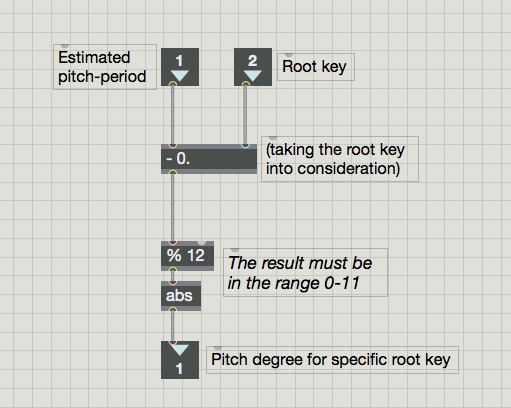
\includegraphics[width=7cm]{Figures/inoctave.png}
\caption{The \emph{inoctave} Max external.}
\label{inoctave}
\end{center}
\end{figure}
\newline
As shown in Figure \ref{inoctave}, we \emph{must} take into consideration the selected root key in order to achieve the right degree value. We have already said that pitch value is \emph{absolute}, i.e. tonality is not considered, and so isn't the octave. We should consider whatever octave and give 0 to the lower considered value, that is the \emph{tonic}. In doing that, we have to convert the root key itself in pitch value and subtract it to the estimated one. For instance, if we have $D$, or 2 in pitch value, and the root key is $C$, its degree value will be 2, the supertonic. On the other hand, if the root key is $D$, we have previously subtracted 2 to the estimated value and so its degree value now is 0, i.e. it's the tonic.
The modulus operator let the result always remain in the established range $0 - 11$, as the pitch class set wants. The value found inside this Max external is the pitch period harmonic function and will be used to select the specific chord the Intelligent Harmonizer will use for this note.

%2. harmonisation control stage
\subsection{Chord selection control stage}
\label{harmonisation}
\begin{figure}[htbp]
\begin{center}
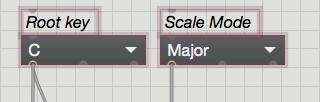
\includegraphics[width=5cm]{Figures/root-key.png}
\caption{\emph{Root key} and \emph{scale mode} parameters.}
\label{harm-param}
\end{center}
\end{figure}
The second parameter shown in Figure \ref{harm-param}, \emph{scale mode}, determines in which manner the harmonisation takes place. Here, the user can switch between different typologies of harmonisation. Each of this has its own musical character, with its own chordal voices displacement:
\begin{itemize}
\item \emph{Major} mode provides a major-scale based harmonisation, while the chords built on the external notes are generally Dominant 7th so to create a like-\emph{tonicization} effect;
\item \emph{Minor} mode provides a blended minor-scale based harmonisation. In fact, we take into consideration two of its versions: \emph{natural} minor and \emph{melodic} minor. Furthermore, they are melt together so to give the user more than one scalic combination. Chords for both natural and melodic 6th and 7th degree are provided.
\item \emph{Blues} mode provides a harmonisation for degrees that form the so-called \emph{pentatonic} scale with the inclusion of augmented 4th degree in a manner that resembles a classic blues scale harmonisation. No chords for notes that are not part of this scale are given.
\item \emph{Parallel} mode gives the user the classic Harmonizer effect. For every octave semitones an equal harmonic function is given, so to create a constant parallel movement of chordal voices. 
\item \emph{Colours} mode is a slightly different one. In fact, it gives the user very \emph{coloured} chords like suspended chords or add chords, that is a triad with the inclusion of what is not a triadic interval (2nd, 4th or 13th interval for instance). As the name suggests, this kind of harmonisation can be useful when the user is expecting a more subtle and discreet sound, or an ambiguous one.
\end{itemize}

\textbf{The \emph{chords} collection.}
How is the chord correctly chosen? We said previously that a chord configuration is made of 4 pitch values. All the chord configurations are set by software designer and stored into a text file, whose name is \emph{chords.txt}, as shown in Figure \ref{coll}.
\begin{figure}[htbp]
\begin{center}
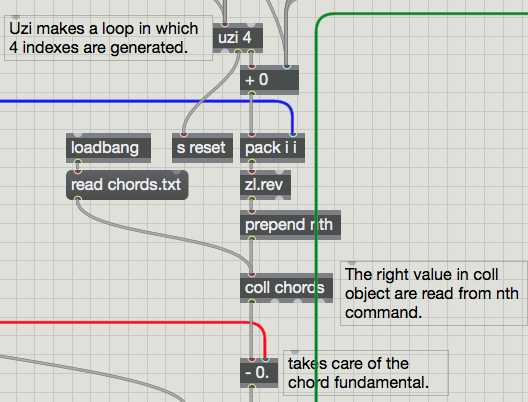
\includegraphics[width=8cm]{Figures/coll.png}
\caption{Harmonisation core stage.}
\label{coll}
\end{center}
\end{figure}
This text file is loaded immediately at the initialisation of the patcher (this is done using the \emph{loadbang} object). The file is made of rows and columns. Each row contains all the different chords that may be selected depending on the \emph{scale mode} choice. The number of rows is equal to the number of semitones that an octave interval can contain. The columns should be read in groups of 4 because we're talking about harmonisation by chords of 4 notes. When the pitch-period harmonic function is recognised, a bang is generated together with the pitch degree value. This bang triggers the \emph{uzi} process, that is to generate a specific number of indexes at the least time amount. These one, together with the pitch degree value, are packed two at a time to make 4 couples. One of these lists contains two integer values: the first refers to the momentary harmonic function of the incoming signal, the second refers to the column in which there's a chord voice it has to be extracted. As the root key and the detected pitch-period, also this voice is in pitch value. The extraction process is made by the \emph{nth} coll argument. It allows for two values, the row one first and the column one then.

Once the desired voice is selected inside the \emph{coll} object, we have to take care about the chord fundamental. For instance, if we have a $G$ note and its harmonic function is dominant, we're expecting messages like \emph{nth 7 0}, \emph{nth 7 1} and so on - for convenience, we're assuming root key is $C$ and scale mode is Major. The pitch values these messages are going to select are 2, 5, 7, 11. These are still not the correct values because we're not taking into consideration that the chord configuration is simply given assuming $C$ as fundamental, as said in \ref{recognize}. What we must do is subtract the pitch-period scale degree to each selected values. Doing this, the new pitch values will be -5, 2, 0, 4. These are the correct values we could pass to the next stage in order to calculate the ratios for pitch shifting engine. In fact, both the lists refers to the same chord: one with $C$ as fundamental, the other with $G$ - that is our case.

%3. 'Intellichord' function
\subsection{The 'Intellichord' function}
\label{intelli}
%cita provenienza Intellichord label
One of the main limitation of a so-built harmonisation is the lack of variation in chord succession standing on the same scale degrees. For instance, using the scale modes presented above there's no difference if the user plays a II - V harmonic succession or its inverted V - II. This is quite wrong, because a musician naturally tends to harmonise differently depending on what particular succession he's playing in. For that reason, he'll harmonise differently a II if he comes from a VI rather than if he comes from a IV. The modes discussed before don't allow it. Naming it, inspiration has taken from the similar function implemented in Carmine-Emanuele Cella's \emph{Revoice}. This software has been described in \ref{subsec:time}.

Here, a different harmonisation mode that tries to care for this musical aspect is shown in Figure \ref{intelli}.
\begin{figure}[htbp]
\begin{center}
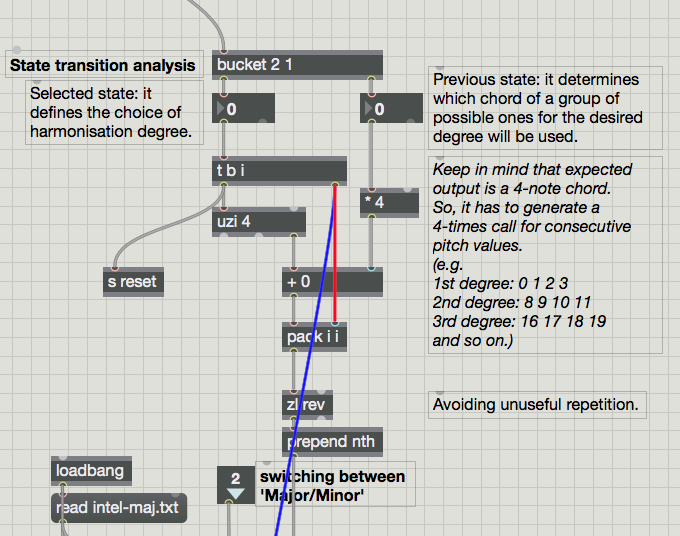
\includegraphics[width=10cm]{Figures/intelli.png}
\caption{\emph{Intellicord} engine.}
\label{intelli}
\end{center}
\end{figure}
As we could see, the process of chord selection in \emph{Intellichord} section is somewhat similar to the other one. The main differences are located before the \emph{uzi} process takes place and inside the text file that is read into the coll object. 

Let's consider the first different aspect.
The detected pitch scale degree comes into the \emph{bucket} object. This allows \emph{Intellichord} to examine every state transition between consecutive chords. In fact, before passing to a next chordal realisation the system takes memory of what scale degree it has just harmonised. Two different states (i.e. degrees) are considered at the same time. The present state defines which harmonic degree the input note is, as it's in the standard section. The previous state determines which chord of a group of possible will be used. Also this collection takes messages with the \emph{nth} argument, and for this purpose lists are created in a similar manner.

Now let's consider the text file structure:
\newline
\begin{table}[htdp]
\caption{The \emph{intelli-maj.txt} file structure.}
\begin{center}
\renewcommand{\arraystretch}{1.2}
\begin{tabular}{p{1.3cm}| p{1cm} p{1cm} p{1cm} p{1cm} p{1cm} p{1cm} p{1cm}}
\ & I & II & III & IV & V & VI & VII \\
\hline
1 & I-1 & II-1 & III-1 & IV-1 & V-1 & VI-1 & VII-1\\
2 & I-2 & II-2 & III-2 & IV-2 & V-2 & VI-2 & VII-2\\
3 & I-3 & II-3 & III-3 & IV-3 & V-3 & VI-3 & VII-3\\
4 & I-4 & II-4 & III-4 & IV-4 & V-4 & VI-4 & VII-4\\
5 & I-5 & II-5 & III-5 & IV-5 & V-5 & VI-5 & VII-5\\
6 & I-6 & II-6 & III-6 & IV-6 & V-6 & VI-6 & VII-6\\
7 & I-7 & II-7 & III-7 & IV-7 & V-7 & VI-7 & VII-7\\
\end{tabular}
\end{center}
\label{intellitable}
\end{table}
\newline
As shown in Table \ref{intellitable}, the first column indicates which scale degree we are moving from, while the first row indicates which scale degree now has to be considered. There's an implicit clockwise movement, whose final point is the cell that contains the chord that will be used for that specific succession. For instance, if the user would move from II to V, \emph{Intellichord} is going to select the chord inside the cell V-2. If the user was moving from IV to I, \emph{Intellichord} would use the chord in cell I-4. Initials inside every cell show the state transition we're talking. Roman numbers indicate the present state, arabic numbers the previous state. 

The main feature of this organisation is that there are 7 possible chords for every harmonic function the device may use, supposing all the state transitions between every scale degree are allowed. This leads to a matrix made of $7 \cdot 7 = 49$ different combinations, and so a greater dynamism in harmonising an incoming signal. Obviously, also the chord configuration in this file is given in pitch values. Differently from the \emph{chords.txt} file, here the chord fundamental is taken into account. 

\section{Interface and performance}
\label{performance}
Now, let's have a quick look at the controls provided to the user for better helping him during a performance situation.


%1. input signal control stage
\subsection{\emph{General Parameters} control stage.}
One aspect the user should notice is that the interface is well-divided into general sections. The first section presented herein, \emph{General Parameters}, contains the most important and basic controls over the entire device.
\begin{figure}[htbp]
\begin{center}
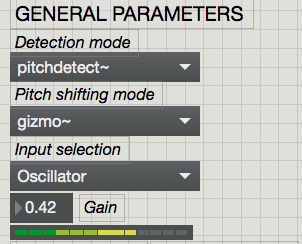
\includegraphics[width=5cm]{Figures/general.png}
\caption{\emph{General Parameters} interface section.}
\label{general}
\end{center}
\end{figure}
Here, the user can switch between several different pitch estimation algorithms. 
\newline
At the present moment, there are two pitch detection algorithms. One, pitchdetect$\sim$, is made by the Author and the Supervisor and its features are well-described in \ref{pitch}. The other, pitch$\sim$, was developed in 2001 by Tristan Jehan and is based on another MSP external, fiddle$\sim$, originally developed by Miller Puckette in fall '90s \cite{puckette1998real}.	
Moreover the user can switch between two different pitch shifting algorithms: gizmo$\sim$ and dlshift$\sim$. As the second has been discussed previously in \ref{dlshift}, \emph{gizmo} is included directly inside Max 7. This object implements a frequency-domain pitch shifting (see \ref{subsec:freq}).
\newline
The concept on which the selection has been done is to give the user the chance to choose and try at least one algorithm for each approach, both for pitch estimation and for pitch shifting. All the algorithms built and discussed in this project works in the time-based approach, instead the other belong to the frequency-domain approach.

Finally, the user is given the control over three different input signal modes: \begin{itemize}
\item \emph{External} allows for real-time performance. In fact, this choice lets the Intelligent Harmonizer take any signal coming directly from an input device, e.g. a microphone or an instrument. The input device is previously set into the Max \emph{Audio Status} window;
\item \emph{Audiofile} is the option the user has to select if he wants to harmonise some audio sample;
\item \emph{Oscillator} feeds the device algorithms with a sine oscillator, whose frequency can be manually controlled via MIDI controller or via the device itself. In fact, when choosing this option a window that shows a virtual keyboard will open. The user may change the oscillator frequency selecting the note onto this keyboard. 
\end{itemize}
Also a gain control is provided. The user can adjust the input signal amplitude looking at the level meter and finding the desired one.

%2. beyond harmonisation: delay and modulations
\subsection{Beyond shifting: \emph{delay} and \emph{modulations}.}
The following section gives some features that may help the user to achieve a better harmonisation experience. 
\newline
\begin{figure}[htbp]
\begin{center}
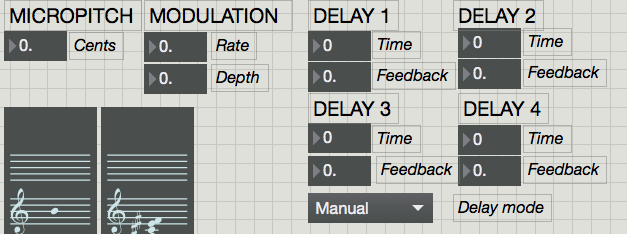
\includegraphics[width=9cm]{Figures/modulations.png}
\caption{The \emph{modulation effect} section.}
\label{mods}
\end{center}
\end{figure}
\newline
As shown in Figure \ref{mods}, the user is given two effect typologies: \emph{delay} effects and based-\emph{modulation} effects.
Delay can be used in several ways. First of all, it can replicate the character of a small vocal group in which the notes of a chord surely don't start at the same moment. It acts producing a \emph{smeared} chord attack. Every singer has his own characteristic vocal emission, and also the \emph{envelope} is involved. Moreover, the singer's own reaction time can affect the moment in which the vocal emission starts. In order to smooth the chord attack and to allow for a more natural-feel sound, each voice has its own delay with unique \emph{length} and \emph{feedback} controls. The first control is the key for achieving the effect mentioned above, and also true delay effects if the delay time overcomes small values, e.g. those in the range 20 - 80 ms. The second control produces interesting arpeggios effect \cite{lazzarini2010audio} and can also produces an interesting \emph{blurred} harmony effect. Feedback retains a small portion of the just harmonised note into the delay line, while a new harmonisation is passing through. This generates a blend between notes that belong to different chords and harmonic contexts: a sort of \emph{impressionism} in music. If we're thinking at the delay time parameter in a creative way, it's possible to realise rhythmic patterns simply providing all the delays with different and audible time settings. Finally, a \emph{historical} parameter that comes from Eventide H9 \emph{Quadravox} pitch shifting algorithm has been included. Switching this control from \emph{Manual} to \emph{Fixed}, the four delays aren't independently variable any more. In Fixed mode, the Delay 1 Time affects all the other ones in a manner that makes Delay 2 Time be longer than Delay 1, Delay 3 Time longer than Delay 2, and so on.

\emph{Modulation} provides an LFO that can be used to achieve a classic \emph{vibrato} effect. It consists of a periodic shifting that tends to simulate the natural imperfections of the vocal emission, and also the particular effect a musician can get on his instrument (for instance, by modulating a guitar string, or using the whammy bar on an electric guitar). We also can think of a vibrato as a vocal technique that comes from a spontaneous nervous tremor in the diaphragm and that can be improved and used on purpose to add expression in music. Since vibrato is typically characterised in terms of amount of pitch variation (that is, the \emph{extent} of a vibrato) and the speed at which the pitch is varied (the \emph{rate} of vibrato), the interface gives the user two independent controls: \emph{depth} and \emph{rate} \cite{cipriani2009musica}.

\emph{Micropitch} is what in Eventide's H910/H949 Harmonizer models was called \emph{Fine Control}. In particular, this control allowed for fine adjustment around Unison when the Micro mode was selected. But generally, this control affected the general pitch shifting ratio controls. Here, the concept of micropitch is quite different. The selection of the ratios, that has been described in \ref{harmonisation}, is not altered. More specifically, this is an addition to the calculated ratios. The control allows for a $\pm50$ cents adjustment and all the voices are affected in the same mode.

%3. output control stage
\subsection{Output control stage.}
\newline
\begin{figure}[htbp]
\begin{center}
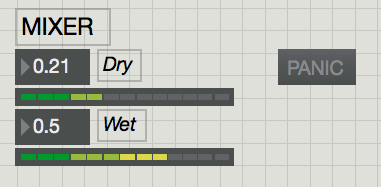
\includegraphics[width=7cm]{Figures/mixer.png}
\caption{The \emph{Mixer} section.}
\label{mixer}
\end{center}
\end{figure}
\newline
Finally, the interface gives the user the control of the level of harmonised sound (\emph{wet} parameter) and direct signal (\emph{dry} parameter). Both the parameters are given in linear amplitude, that is, they range from 0 (no sound) to 1. No gain in this stage is allowed because the user can directly act both on the input level and on each of harmonisation voices if he wants to raise the overall level.
It's also provided a useful \emph{panic} button. If pushed, it stops immediately all the DSP processes and neither input nor output signal can be heard. To restore the correct function of the device, the user has to be start again the DSP engine from the Max \emph{Audio Status} window. In order to prevent undesired sounds when DSP is turning on again, \emph{panic} makes all the input and output levels set to their minimum.

\section{Issues and future enhancements}
\label{future}
%aggiungere: pitch shifting con delay line � metodo debole. opportuno sostituire con algoritmi pi� potenti, quali ad esempio PV o PSOLA;
%aggiungere: AMDF pu� generare errori di pitch detection in casi di materiale critico; opportuno studiare implementazioni pi� robuste che limitino la possibilit� di errore;

%musical aspects improvements
Harmonisation process is a very personal one. Numerous treatises on music harmony have furnished many students different ways of harmonic realisation. There has been no definitive formalisation until now. 
As Piston wrote in \cite{piston1978harmony}:
\begin{quote}
\scriptsize{True harmonisation, then, means a consideration of the \emph{alternatives} in available chords, the reasoned selection of one of these alternatives, and the tasteful arrangement of the texture of the added pans with due regard for consistency of style. (p. 152)}
\end{quote}
Surely, the idea of harmonisation including specific musical style codified aspects is not the aim of this work. Generally, a Harmonizer has often been seen as a way of getting a quickly harmonisation and there has been not so much attention on the quality of its realisation, considering not the technical but rather the musical aspect. As shown in \ref{harmonisation}, also this device does not pay attention in the choice of arrangement and in the choice of a better alternative chord relative to the context. In fact, what our Harmonizer does is to read a table and get out the selected pitch values. If the \emph{scale mode} is changing, the selected chord will be different. But, internal to a specific harmonisation mode, there's no alternatives in available chords. This means that, for the same note, the same chord will always be selected. Moreover, there's no attention to any melodic lines as it should be in a classic four-voice writing. The concept of \emph{mutual connectibility} exposed by Piston in his own manual is not considered. In practice, most of the musical aspects and heuristics for an appropriate harmonisation are missing. This is a normal issue regarding many harmonizers, due to the fact these devices should be first very accessible to a vast range of utilisers and are affected by all the computing and technology limitations.\\
A first attempt to solve this lack of musical considerations can be seen in the development of our \emph{Intellichord} function, as shown above in \ref{intelli}. This harmonisation mode does not care about style or any arrangement taste, but focuses on the recognition of the state transitions in order to make a reasoned selection inside a range of several alternative chords. 

%1. more strategies in achieving interesting harmonisations?
\subsection{Probabilistic networks?}
In the recent time, the research focused on non-deterministic approaches and on the use of logical and mathematical assumptions in order to obtain more sophisticated harmonic realisations in a manner that can take into account a pseudo human experience. In fact, Artificial Intelligence is not able to capture the musical style of a human composer \cite{boltzmann1994}, and all his symbolic representations. This symbols make a particular rule be effectively good to describe a specific musical character, that is the \emph{style}. So, more and more diffuse is the use of probabilistic frameworks or the use of neural systems that allow to create a harmonisation system which ``\emph{learns} from examples'' \cite{allan2005harmonising} and experience. In particular, we'll provide a short description of two of these.\\
The first uses a data set of chorale harmonisations to train a Hidden Markov Model. This learning task allows to build a model of harmonic processes that can be used to compose novel harmonisations that follow particular aesthetic preferences of a wanted style, due to the clearly understanding of the basic rules of harmonisation \cite{allan2005harmonising}. The second uses neural networks both in training task and in the harmonisation process. In particular, it's been designed a learning system based on the Boltzmann Machine which allows to learn a particular harmonisation style \cite{boltzmann1994}. The same system can be used with adjustment and constraints (that is, the harmonic \emph{rules}) to harmonise music via completion.

%discussion over probabilistic networks
We can observe how the examples are focused mainly on two characteristics. First, both of the processes are non-deterministic and based on probabilistic networks. This means that there are not pre-configured tables of chords, as it's our case. The system makes a choice between different combinatoric possibilities, looking for the one that better suits the requested harmonisation. This process depends both on the nature of the melody and on the stochastic nature of the models involved (Boltzmann distribution, or Markov Model for instance). We can speak in some way of a real harmonic \emph{synthesis}. This also makes the system perform different results even if the melody is the same. Secondly, both of the examples allows for machine-learning music harmonisation systems. Given the advance in machine learning, it's desirable to apply its techniques to music harmony so to build a system that learns to harmonise and to distinguish between different musical styles. So, the great advantage of this networks is that they are capable of learning internal representations and are also able to solve difficult combinatoric problems. Doing so, the chord construction and its displacement over four voice is truly a real-time task. 

Perhaps, one issue about Boltzmann Machine is that it could stop learning correctly. Learning in general Boltzmann Machine is quite impractical, so it could be made useful to properly constrain the connectivity. This means to insert external constraints in order to let the process efficient enough, whereas the Hidden Markov Model example learns its harmonisation constraints directly from training data. These external constraints are vital to the success of the Boltzmann Machine harmonisation system. Moreover, neural networks are less compute-intensive, but these harmonisation systems retain a pre-programmed knowledge base \cite{allan2005harmonising}. They take a large set of rules written by a human, and so could penalise undesirable combinations of notes so that they can be filtered out. Instead, Markov models don't need predetermined tune or implicit control knowledge.

In conclusion, several system have applied probabilistic networks to harmonisation. Using these kind of system allows to perform more efficient inference to generate new harmonisations. It's also possible to let the system itself learn from adequate examples provided by an external user. In this manner, learning processes and techniques takes importance as much as the harmonisation process itself. The choice of right notes to complete a specific chord and the choice of which harmonic formulae the system should use in a specific content should be made by stochastic models. They allow for non-repetitive patterns, even if the harmonised material doesn't change. In a musical view, these characteristics would be a truly improvement for this kind of device. They perhaps require lots of non-musical knowledge, as most of the concepts come from mathematics and statistic. Further information about HMM-based harmonisation model can be found in \cite{ueda2010hmm}, as in \cite{paiement2006probabilistic} different representation for musical chords that are presented. 

\section{Conclusion}
\label{ending}
In this chapter, we focused mainly on the musical aspects of this project.
First, we described the process that lets this Harmonizer be \emph{intelligent}, that is to recognise every pitch-period harmonic function so to give it a specific scale degree, depending on the selected root key. Then, we described the different typologies of harmonisation that the device provides the user, and how the chords are selected. A more accurate harmonisation model, \emph{Intellichord}, is also shown. Later in the chapter, the user interface was shown in details. All its section were described, and also all the effects and controls. Finally, it's been provided a briefly discussion about possible enhancements so to realise a more complete, ready-to-use and sophisticate device. 

At the end of this paper, we can observe that all this work is undoubtedly acceptable. Nevertheless, several improvements and a change for the better are recommended. In particular, the realm of harmonisation system should be enhanced to give it a more flexible behaviour.
The Author wishes for a possible work of revision and improvement during the successive years.





